\csname documentclass\endcsname[../main.tex]{subfiles}
\begin{document}
\chapter{Method}


In this chapter, we document how we propose 
to learn a non-greedy intervention policy.
We first
formalize interventions and intervention policies,
then introduce the surrogate models we use
to calculate intermediate rewards,
and finally, present how Reinforcement Learning is used 
to learn a non-greedy intervention policy.

Building on top of IntCEMs, which augment a CEM
with a greedy intervention policy model and train the two simultaneously,
we propose RLCEM,
a novel CEM model augmented with a Reinforcement Learning agent
that learns a non-greedy intervention policy.
The two are trained simultaneously, similar to IntCEM, 
where the sampled interventions are used to increase the sensitivity of the
$\mathbf{c} \to \mathbf{y}$ label prediction model.

An overview of the general structure of our RLCEM is in Figure~\ref{fig:rlcem-overview}.
The RL agent learns to output interventions, which are 
used to train the CEM to increase sensitivity of 
CEM to interventions. After all interventions from the RL agent,
the CEM prediction is used to calculate the final
reward to train RL agent. Additionally, the surrogate model
is used to calculate intermediate rewards which are used to train and guide the 
RL agent to make more optimal intermediate interventions.
We select Arbitrary Conditional Flow (AC Flow)
models~\cite{acflow} as our surrogate models, and use 
Proximal Policy Optimization~\cite{ppo}
to train our RL agent.

\begin{figure}[!ht]
    \centering
    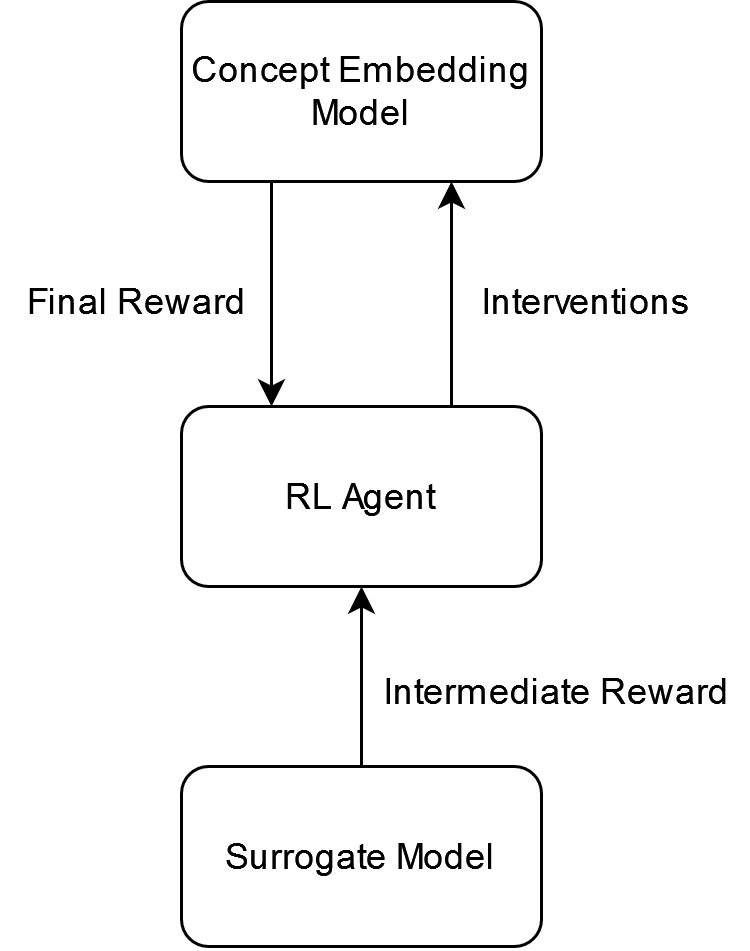
\includegraphics[width=0.4\textwidth]{figs/method/rlcem_overview.png}
    \caption{An overview of the structure of RLCEM. The RL agent samples interventions for the CEM, which is used to calculate
    the final reward to train the agent. The surrogate model is used to calculate intermediate rewards
    to train the agent.}
    \label{fig:rlcem-overview}
\end{figure}

\section{Interventions}
A key advantage of using CBMs is having access to 
run-time interventions, which is the idea of utilizing professionals
to modify incorrect concept predictions to improve the 
performance of the model.
For simplicity, we do not consider incorrect interventions, 
i.e. when the professionals misjudge and modify
 the predicted concepts to incorrect values,
and assume that
all interventions are correct. To formalize interventions, we define
them via the following function, where
the predicted concepts $\hat{\mathbf{c}}$ and the true concepts $\mathbf{c}$ are interpolated
using a multi-hot encoding intervention vector $\bm{\mu}$.

\[I(\hat{\mathbf{c}}, \mathbf{c}, \bm{\mu}) = 
\bm{\mu} \; \mathbf{c} + (1 - \bm{\mu}) \; \hat{\mathbf{c}} \qquad \hat{\mathbf{c}}, \mathbf{c}, \bm{\mu} \in \{0, 1\}^k\]

Figure~\ref{fig:interventions} demonstrates how an intervention
is formed using 
a binary mask $\bm{\mu}$ from the predicted concepts $\hat{\mathbf{c}}$ and the true concepts $\mathbf{c}$.

\begin{figure}[!ht]
    \centering
    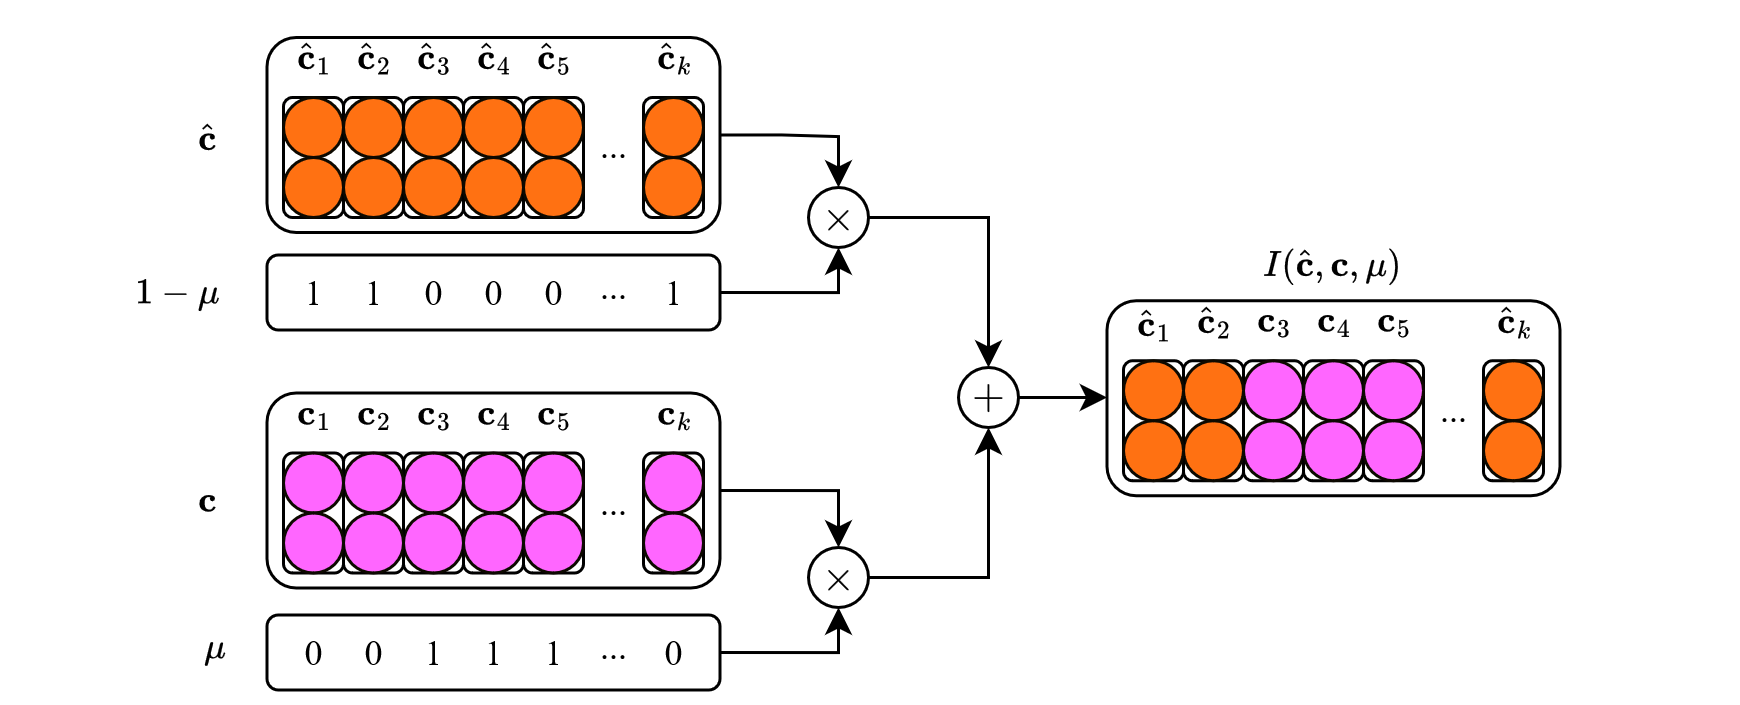
\includegraphics[width=\textwidth]{figs/method/interventions.png}
    \caption{An example of how interventions are formed from the predicted concepts $\hat{\mathbf{c}}$
    and true concepts $\mathbf{c}$
     using binary mask $\bm{\mu}$.}
    \label{fig:interventions}
\end{figure}

\subsection{Intervention Policies}

An intervention policy $\mathcal{P}$ determines the order of concepts to intervene 
on with the goal of maximizing the accuracy of the $\mathbf{c} \to \mathbf{y}$ concept prediction model.
A greedy intervention policy is thus a collection of functions $\mathcal{P}_i$, each
of which outputs the concept to intervene on at step $i$. An optimal greedy policy is the following
\[\hat{\mathcal{P}} = \bigcup_{i=1}^k \mathop{\mathrm{argmax}}_{\mathcal{P}_i} Acc(\hat{g}(\hat{\mathbf{c}}_{\mathcal{P}_j}), \mathbf{y}) \]
% \[\hat{\mathcal{P}} = \mathop{\mathrm{argmin}}_{\mathcal{P}} \sum_{j = 1}^{k} \mathcal{L}_{\text{task}}(\hat{g}(\hat{\mathbf{c}}_{\mathcal{P}, j}), \mathbf{y}) \]
\[\hat{\mathbf{c}}_{\mathcal{P}_0} = \hat{\mathbf{c}}, \hat{\mathbf{c}}_{\mathcal{P}_j} = I(\hat{\mathbf{c}}_{\mathcal{P}_{j-1}}, \mathbf{c}, \mathcal{P}_j(\hat{\mathbf{c}}_{\mathcal{P}_{j-1}}))\]
Which maximizes the accuracy at each step $j$ sequentially
for all $k$ concepts. At each
step, $\hat{\mathbf{c}}_{j-1}$ is 
the predicted concept after the previous $j-1$ interventions,
and we aim to maximize the accuracy of the prediction made by the
$\hat{g}: \mathbf{c} \to \mathbf{y}$ model.


Compared to a greedy intervention policy, a non-greedy intervention 
policy outputs a set of concepts to intervene on for a budget $j$,
which we want to maximize the accuracy of the $\mathbf{c} \to \mathbf{y}$ model on. 
An optimal non-greedy policy maximizes the following
\[\hat{\mathcal{P}} = \mathop{\mathrm{argmax}}_{\mathcal{P}} \sum_{j=1}^k Acc(\hat{g}(\hat{\mathbf{c}}_{\mathcal{P}_j}), \mathbf{y}) \]
\[\hat{\mathbf{c}}_{\mathcal{P}_j} = I(\hat{\mathbf{c}}, \mathbf{c}, \mathcal{P}(\hat{\mathbf{c}}, j))\]

Note that the notion of a budget, defined as the number
of concepts the model is allowed to intervene on for simplicity, is only
meaningful for non-greedy policies. Non-greedy policies aim
to maximize the accuracy of the $\mathbf{c} \to \mathbf{y}$ model after using up the intervention budget,
and may select different sets of intervention concepts 
for different budgets. Greedy policies always select the same
concepts per step and thus the budget does not 
affect the concept selected by the policy.
This is why existing intervention policies do not consider
budgets, and why we consider them in our research question.

% Budget
% In this project, we utilize Reinforcement Learning

\section{Surrogate Models}\label{method:surrogate}

We use generative surrogate models that models the likelihoods of concepts
to guide the RL model. 
Such a surrogate model is needed because
when we are learning
a non-greedy policy, its performance is measured by the accuracy
of the model after all interventions in the end.
When training an RL agent to learn such a policy, this corresponds
to rewarding it at the final step based 
on the final accuracy, and training it to maximize this reward.
% if we were to train an RL agent by rewarding it in the intermediate steps
% this would become a greedy policy.
However, previous studies have shown that
using delayed rewards, where the agent is only rewarded after long episodes,
can pose a challenge to its learning as the agent struggles to learn
the consequences of its actions~\cite{ steps-towards-ai, temporal-credit-assignment},
and thus struggles to learn to make the correct decisions.
Therefore we introduce intermediate rewards 
to guide the RL agent to make the correct intermediate
interventions that lead 
to the largest final accuracy.

Following Li et al.~\cite{afa} in Active Feature Acquisition,
we use a surrogate model 
to approximate
the conditional likelihoods $p(\mathcal{C}_u \mid \mathcal{C}_o, \mathbf{y})$, 
where $\mathcal{C}_u$ is a set of un-intervened
concepts, $\mathcal{C}_o$ a set of intervened concepts,
and $\mathbf{y}$ the label. 
In the context of an intervention, the previously intervened concepts would be $\mathcal{C}_o$,
and the current concept we are intervening on would be
$\mathcal{C}_u$.

We use a variant of the popular normalizing flow models~\cite{normalizing-flows},
namely Arbitrary Conditional Flow (AC Flow)~\cite{acflow}
models as our surrogate models.
These models are 
flow models augmented to model arbitrary conditional likelihoods $p(\mathcal{C}_u \mid \mathcal{C}_o)$
between sets of variables $\mathcal{C}_u$ and $\mathcal{C}_o$.
We extend these models to approximate the class-conditional
likelihoods
$p(\mathcal{C}_u \mid \mathcal{C}_o, \mathbf{y})$. To represent
these sets of concept,
we use concept vectors $\mathcal{c}$ along with
binary masks $b$ and $m$.
The mask $b$ represents
the already intervened concepts, the mask $m$ represents
the concepts we are interested in ($\mathcal{C}_u$ and $\mathcal{C}_o$).
Mathematically this gives us two concept vectors
\[\mathbf{c}_o = \mathbf{c} \cdot b\]
% \[\mathbf{c}_u, \mathbf{c}_o = \mathbf{c} \cdot m\]
\[\mathbf{c}_u = \mathbf{c} \cdot (1 - b) \cdot m\]
For convenience, we use $\mathbf{c}_u$ and $\mathbf{c}_o$ from now on
to represent the sets of concepts $\mathcal{C}_u$ and $\mathcal{C}_o$, with
$c_i \in \mathbf{c}_u, \mathbf{c}_o$ representing the individual concepts.

\subsection{Latent Distribution}

As described in Section~\ref{background:flow}, 
normalizing flow models utilize the change of variable formula to model likelihoods,
which can be extended to include conditional likelihoods. AC Flow models build on
Transformation Autoregressive
Networks (TANs)~\cite{tans}, and learn to model 
likelihoods $p(c_0,\ldots, c_n \mid \mathbf{c}_o ,\mathbf{y})$,
modelling the underlying latent distribution using an autoregressive approach with Recurrent
Neural Networks (RNNs)~\cite{rnn}. The RNN learns to model the likelihood of 
$p(z_0, \ldots, z_n \mid \mathbf{z}_o , \mathbf{y})$ by sequentially processing each of the variables
 $z_i$.
At each step $i$, an RNN outputs parameters for an underlying Gaussian Mixture Model (GMM),
which is a mixture of $K$ different Gaussian distributions~\cite{gmm}.
This allows us to compute $p(z_0, \ldots, z_i \mid \mathbf{z}_o , \mathbf{y})$,
the likelihood of the current $i$ variables,
using a weighted
sum of the probability density of the Gaussian distributions. Experimentally
we find that setting the number of components $K$ to be the number of classes of
$\mathbf{y}$, equivalent to one Gaussian distribution per 
class 
achieves
a good balance between model performance and computational efficiency.
% , which is discussed further in Section~\ref{eval:surrogate}.
While using a GMM does not directly gives us the probability of
$p(z_0, \ldots, z_n \mid \mathbf{z}_o , \mathbf{y})$, 
it allows us to compute the probability density which tells us the likelihood of the
 variables $z_0, \ldots, z_n$, which is proportional
 to the actual probability and also allows us to sample from the distribution.

\subsection{Transformations}
In order to transform latent likelihoods $p(z_0, \ldots, z_n \mid \mathbf{z}_o , \mathbf{y})$ to 
the concept likelihoods
$p(c_0,\ldots, c_n \mid \mathbf{c}_o , \mathbf{y})$, we
utilize a set of transformations with learnable parameters that 
map input concepts $c_i$ to latent variables $z_i$. We follow the 
set of conditional transformations defined by Li et al.~\cite{acflow}, and extend them to
be label $\mathbf{y}$ specific.
These transformations $q_{\mathbf{c}_o, b, \mathbf{y}}$ are
conditional on 
intervened concepts $\mathbf{c}_o$, binary mask $b$, and label $\mathbf{y}$, 
and are invertible so that we can obtain the liklihood and 
sample from the latent distribution. 
For all un-intervened concepts $\mathbf{c}_u$,
the transformation maps these concepts to latent variables $q_{\mathbf{c}_o, b, \mathbf{y}}(\mathbf{c}_u) = \mathbf{z}_u$. 
We can then apply the change
of variable theorem with a conditional extension, and using
the Jacobian determinant tells us how the likelihood changes~\cite{normalizing-flows}.

\[p(\mathbf{c}_u \mid \mathbf{c}_o, b, y) = \left | 
\mathop{\mathrm{det}} \frac{d q_{\mathbf{c}_o, b, \mathbf{y}}}{d \mathbf{c}_u}
\right | p(q_{\mathbf{c}_o, b, \mathbf{y}}(\mathbf{c}_u) \mid \mathbf{c}_o, b, y)\]

In the AC Flow model, we mainly leverage
linear transformations. We use Multi-Layer Perceptrons (MLP)~\cite{feedforward} 
$\phi$ to learn 
a weight matrix $\mathbf{W}$ and bias vector $\mathbf{t}$
\[\mathbf{W}, \mathbf{t} = \phi(\mathbf{c}_o, b, \mathbf{y})\]
As shown in Figure~\ref{fig:linear-transformation},
this gives us a linear transformation for all possible concepts,
and by indexing 
\[\mathbf{W}_{u} = W[1-b][1-b], \mathbf{b}_{u} = \mathbf{b}[1-b]\]
to select the entries corresponding to the un-intervened concepts, we obtain
\[\mathbf{z}_u = \mathbf{W}_{u}\mathbf{c}_u + \mathbf{b}_{u}\]
 This transformation is 
straightforward to invert, and we can find the Jacobian determinant easily and apply the change of variable
theorem illustrated above to get the likelihood $p(\mathbf{c}_u \mid y)$.
Other variants, such as using an RNN to learn a linear transformation
for each , are also included to add flexibility to the transformations such that
we are able to model the input data distribution. More details on the transformations
we used can be found in Appendix~\ref{appendix:transformations}.

\begin{figure}[!ht]
    \centering
    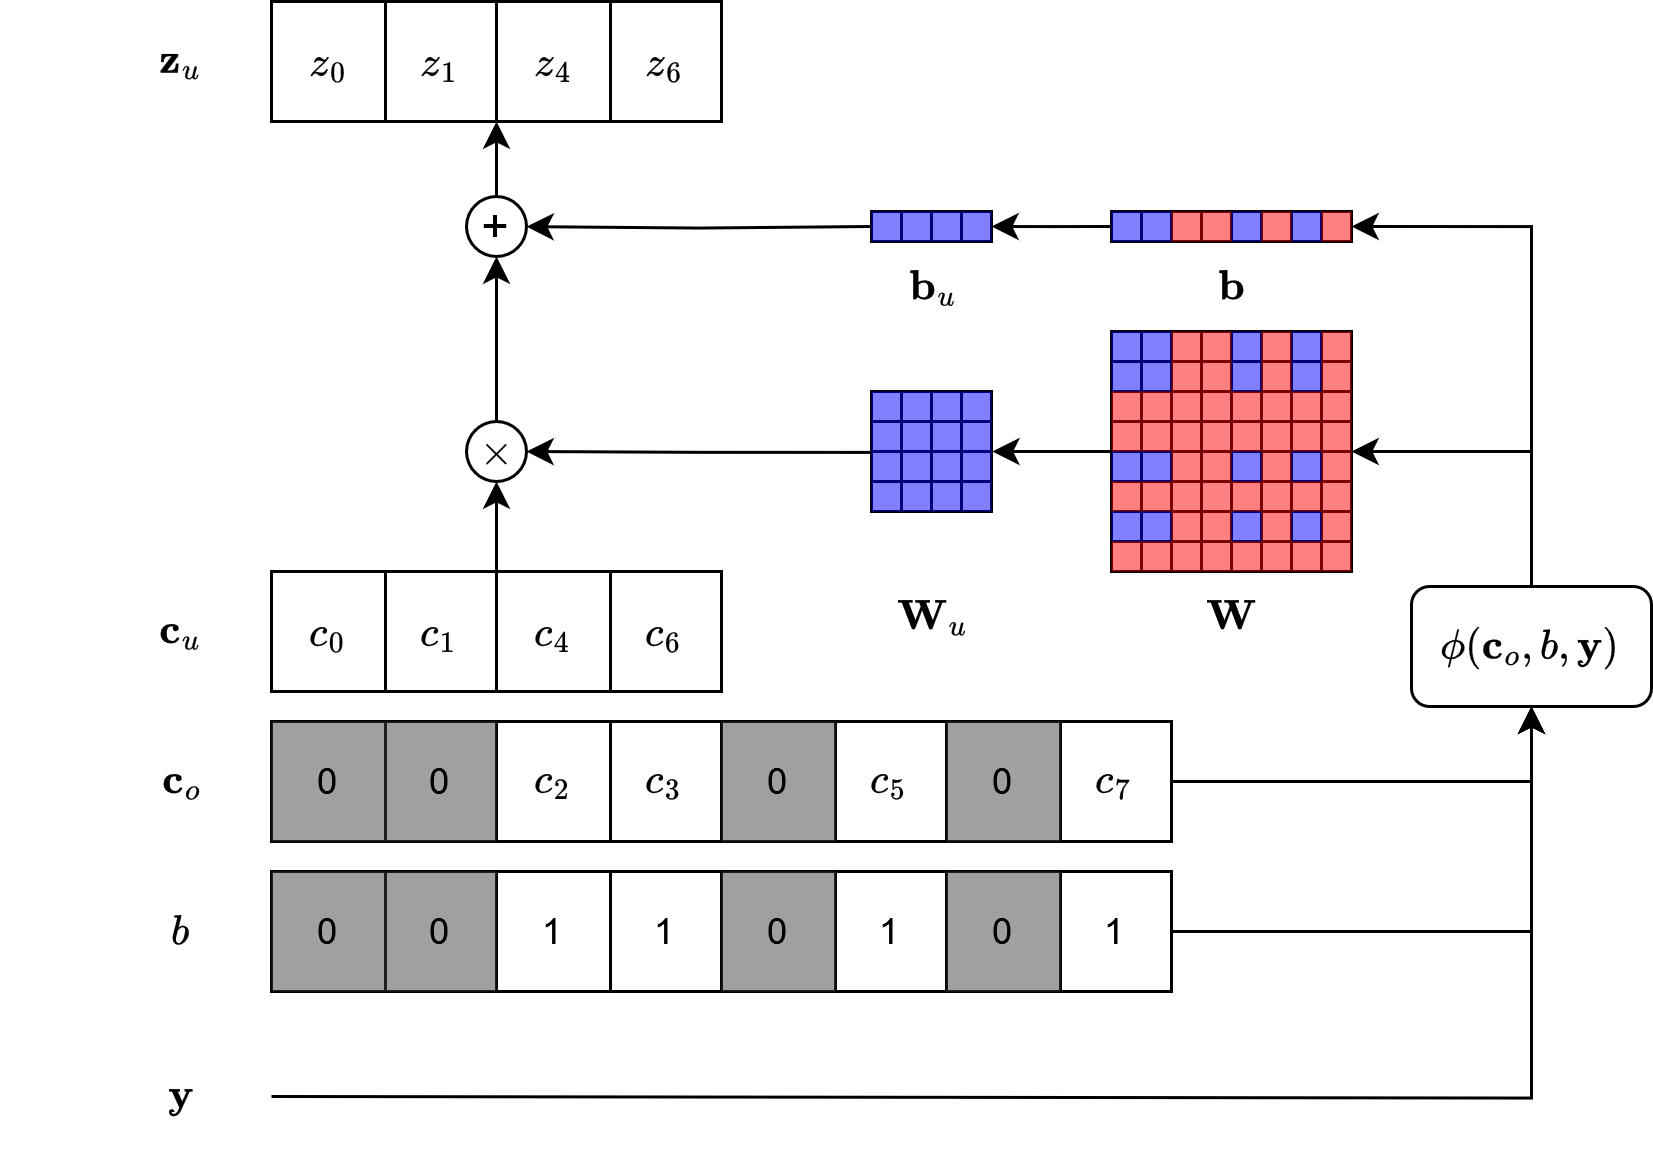
\includegraphics[width=0.8\textwidth]{figs/method/transformations.png}
    \caption{An example of linear transformation.}
    \label{fig:linear-transformation}
\end{figure}

These tranformations and the latent distribution are both learnt to
approximate the conditional likelihoods $p(c_0, \ldots, c_n \mid \mathbf{y})$
or the likelihood of seeing a set of concepts $p(\mathbf{c}_u \mid \mathbf{y})$.
% seeing a set of unobserved concepts $\mathbf{c}_u$
% given a set of observed concepts $\mathbf{c}_o$ and a class $\mathbf{y}$. 
By using Bayes' theorem, we note that
we can additionally model the conditional likelihoods of the label and un-intervened
concepts
\begin{equation}\label{equation:bayes}
p(\mathbf{y} \mid \mathbf{c}_o ) = \frac{
p( \mathbf{c}_o \mid \mathbf{y}) P(\mathbf{y})}
{\sum_{y'} p( \mathbf{c}_o \mid \mathbf{y}')P(\mathbf{y}')}
\end{equation}
Which the right hand side terms can be computed using the AC Flow model, with
$p(\mathbf{c}_o \mid \mathbf{y}) = p(\mathbf{c}_o \mid \emptyset, \mathbf{y})$, where we 
use an empty set of concepts as the condition.
As we can see in Section~\ref{method:rlcem}, this likelihood is used to 
provide rewards to the RL agvent.

Since the transformations learnt are invertible,
we can also sample from the data distribution
via the underlying distribution.
% Due to the invertible property of the learnt transformations,
% a model learnt this way also allows us to sample from the underlying probability 
% distribution then applying the transformations, which gives us 
% samples from the input distribution.
This is useful for the RL agent to
determine interventions as
this provides information on which concepts are likely to be present 
(or not present) given the currently intervened
concepts.

In general, we follow the advised hyperparameters from Li et al.~\cite{acflow}
for building the transformations used in our AC Flow model. This includes the rank of the linear
matrices $\mathbf{W}$ and the hidden dimension of the latent distribution RNN. 
% However, we notice that while
% they use $k \times m$ components in the Gaussian Mixture Model where $k$ is the number of concepts
% and $m$ is the number of classes, we can use $m$ components without any noticeable performance drop.
% Sufficient transformations are required for the AC Flow model to 
% approximate the data distribution accurately, and we do not change them.

\subsection{Training the Surrogate Models}\label{method:training-surrogate-model}

In this project, we adapt AC Flow models to model the likelihoods of concepts in CEMs during interventions.
We follow the description of Li et al.~\cite{afa} and implement corresponding AC Flow models to model
the distribution of concepts.

We train the AC Flow models using a combination of two losses, a negative
log likelihood loss and a mean-squared error (MSE) loss . 
Since these models output likelihoods directly,
we can directly maximize the likelihood, or equivalently minimizing the negative log likelihood.
Additionally, a cross entropy loss is incorporated to help the model
learn the conditional likelihood with respect to the label $y$. 
Given $\mathbf{c}_u, \mathbf{c}_o, y$, we compute the class with the highest likelihood
$\hat{y} = \mathop{\mathrm{argmax}}_y p(\mathbf{c}_u, \mathbf{c}_o \mid y)$ and compute 
a cross entropy loss $CE(\hat{y}, y)$ such that the model learns to 
output higher likelihoods for concepts that belong to the correct class.
The loss thus becomes
\[Loss = - \log p(\mathbf{c}_u \mid \mathbf{c}_o, \mathbf{y}) +
 CE(\mathop{\mathrm{argmax}}_\mathbf{y} p(\mathbf{c}_u, \mathbf{c}_o \mid \mathbf{y}),  \mathbf{y})
\]
Additionally, we add a penalty term to the loss to prevent 
the model from outputting large values of likelihoods in general.
To penalize
large values, similar to an L2 regularization loss,
we add the square of the logits $\log p(\mathbf{c}_u, \mathbf{c}_o \mid \mathbf{y})$ and 
$\log p(\mathbf{c}_o \mid \mathbf{y})$
to the loss. 
This penalty term is further discussed in 
Section~\ref{eval:surrogate}. 
The final loss for training the
AC Flow model is
\begin{align*} 
Loss = & - \log p(\mathbf{c}_u \mid \mathbf{c}_o, \mathbf{y}) + 
CE(\mathop{\mathrm{argmax}}_\mathbf{y} p(\mathbf{c}_u, \mathbf{c}_o \mid \mathbf{y}),  \mathbf{y})
\\ & + \lambda_{l2} \left ( \log^2 p(\mathbf{c}_u, \mathbf{c}_o \mid \mathbf{y}) + 
\log^2 p(\mathbf{c}_o \mid \mathbf{y}) \right )
\end{align*}


\section{RLCEM}\label{method:rlcem}

% Talk about how the RLCEM model is formed
% The goal, losses etc
% Detailed description of what happens during training and testing
% Diagram
% Talk about design choices: num_rollouts, batch_size sampling of budget etc
Instead of using 
the original CBMs as our base models, we adopt CEMs as they have been shown to have
better performance with and without interventions compared to CBMs~\cite{cem}.
Additionally, CEMs are more robust to concept-incompleteness, 
which is when the concepts present 
in the dataset annotations do not contain all possible concepts
that can be used to, an important issue in real-life datasets. This is because
CEMs learn to output intermediate
concept embeddings rather than binary values~\cite{cem}.

We construct RLCEMs by augmenting CEMs with an RL agent as 
described below, which is our proposed
solution to our main research question.

% We compare our RLCEM against IntCEM and other SOTA intervention policies, which
% are evaluated on the datasets described in~\ref{method:datasets} and we report
% the intervention performance.

\subsection{Reinforcement Learning}\label{method:rl}

We model the problem of finding a non-greedy intervention policy as a 
Reinforcement Learning problem. As mentioned in Section~\ref{background:rl},
Reinforcement Learning is used to find non-greedy solutions to problems
by design as it models the long-term effects of its actions, and aims to 
maximize the overall reward gain. 

In order to formulate the problem
as a Reinforcement Learning problem, we model the problem
of deciding the concepts to intervene on  
as a Markov Decision Problem~\cite{rl-mdp}.

\textbf{States} comprise of the information available
    at each step. This contains the remaining budget and 
    state of the CEM, including its bottleneck and predicted concepts.
    This also contains the output of the surrogate model, 
    including the sampled values for the un-intervened concepts 
    $\bar{\mathbf{c}_u} \sim p(\mathbf{c}_u \mid \mathbf{c}_o, \mathbf{y})$,
    $\bar{\mathbf{c}_u} \sim p(\mathbf{c}_u \mid \mathbf{c}_o)$
    from the class-conditional and marginalized likelihoods
    as described in Section~\ref{method:surrogate}.

\textbf{Actions} correspond to performing interventions 
on the un-intervened concepts.
For simplicity, we group concepts into groups, and each action intervenes on all concepts
within a group.

\textbf{Rewards} are the increase in 
    information, calculated using entropy, to the target $y$~\cite{afa} given by
    \[\text{Reward} = H(y \mid \mathbf{c}_o) - \mathbb{E}_{p(\mathbf{c}_u \mid \mathbf{c}_o)} [H(y \mid x_u, x_o)]\]
    This is because we want to encourage the RL agent to make interventions
    that provide more information to the target variable, or reduce uncertainty, an idea that has shown
    to work well in CooP~\cite{coop}.
    Simplifying gives us
    \[\text{Reward} = H(\mathbf{c}_u \mid \mathbf{c}_o) - 
    \mathbb{E}_{p(\mathbf{y} \mid \mathbf{c}_o)} [H(\mathbf{c}_u \mid y, \mathbf{c}_o)]\]
    which can directly be calculated from the output of the surrogate model using Equation 
    ~\ref{equation:bayes}.
    The final reward when the sequence terminates 
    should reflect how well the prediction post-intervention is.
    It is calculated as negative of the Cross Entropy Loss, where a higher value corresponds to 
    a lower discrepancy between the predicted label and the true value. 
    As this requires knowledge of the true label,
    this reward is only computed during training to train the RL agent. 
    This is also the reason why
    Reinforcement Learning is unable to learn a greedy intervention policy as this would
    require knowledge of the ground truth label at each step to compute the intermediate rewards.
    Li et al.~\cite{afa} 
    also show that using this intermediate reward will not affect the optimality of the learnt policy.
    Using these two rewards
     results in an RL agent that learns to balance between making interventions that
    increase the information to the target variable, which should lead to better final accuracy,
    and other types of interventions that also result in a higher final accuracy.

    
\textbf{Termination} is when the remaining budget is insufficient for more interventions.
    
% In order to decide when to terminate, 
% To model the budget and costs for the interventions, we come up with two approaches:

To model budgets and acquisition costs, we can either

\begin{enumerate}
    \item Incorporate the acquisition costs for each concept into the reward by subtracting
    the corresponding cost. The RL agent
    learns to balance automatically intervening on concepts that are more costly versus the
    potential extra reward gained by the increase in information and accuracy. The RL agent then determines when to terminate
    if the cost of intervening on new concepts outweight the potential gain.
    \item Or leave it out of the reward, such that
    the reward only contains the information gain in each step. 
    We manually step to the termination
    step if and only if the the remaining budget does not allow for future interventions.
\end{enumerate}

The first approach
involves balancing the weights between the intervention costs and reward, and does not 
adopt to the idea of budgets very well, and we select the second approach.
To further simplify, we assume that all concept groups have the same cost
to intervene on. Thus we set the cost of each intervention to be 1, and the budget
becomes the number of possible interventions.

\subsection{Training the agent}

In Active Feature Acquisition as described in Section~\ref{background:afa},
Li et al.~\cite{afa} combine Reinforcement Learning with 
AC Flow models to find the optimal features to acquire 
from the environment. We
adopt a similar approach to train the RL agent.

We first pre-train an AC Flow model that learns 
arbitrary conditional likelihoods about the underlying
concepts $p(\mathbf{c}_u \mid \mathbf{c}_o, y)$. 
Then, A Reinforcement Learning agent is trained to maximize 
the reward given in Section~\ref{method:rl}. 
At each
step, the agent is given the current intervened concepts $\mathbf{c}_o$, 
and then the agent samples the next 
concepts to intervene $\mathbf{c}_u$, 
where the agent is rewarded based on the expected information gain
to the target variable.
At each step, the agent has access to the sampled un-intervened concepts $\hat{\mathbf{c}_u}$ 
from the AC Flow model. This allows the RL agent to learn to intervene on concepts that are 
more likely incorrectly predicted.

Compared to Active Feature Acquisition, the problem setting is a lot more complex as
rather than simply acquiring features from the environment, we are trying to determine
which concepts are more likely to be incorrectly predicted by the $\mathbf{x} \to \mathbf{c}$ model, 
and
which concepts are more likely to, when corrected, guide the model towards the correct prediction
 $\mathbf{y}$.
Additionally the goal is to train one RL agent to be able to determine which concepts
to intervene on for different budgets, which adds another layer of complexity as we require
one unified model for the different tasks with different budgets.

\subsection{Reinforcement Learning Algorithm}

As mentioned in Section~\ref{background:rl}, the state-of-the-art RL algorithm 
for learning
a policy is Proximal Policy Optimization (PPO)~\cite{ppo}, which we use
to train a RL agent that learns a non-greedy intervention policy.
PPO utilizes a Critic model to estimate
the value of a particular state, which is the discounted expected future rewards. Then
an Actor model learns a policy
for taking actions that lead to states with higher values as estimated by the
Critic model.

During training, a state and its true value is computed
and compared to the estimated value by the Critic, and a value loss is computed to minimize
the discrepancy between these two values. Then a policy loss is computed
by the discrepancy between actions selected for states and the estimated
change in value by taking that action.
Ultimately, the Critic model
should be able to estimate the value of a state which reflects
its future label prediction accuracy after all interventions,
and the Actor model should be able to estimate the optimal policy, 
which is the interventions that lead to the highest label prediction accuracy 
after all interventions.

\subsection{Combining RL with CEM}

Zarlenga et al.~\cite{intcem} showed that combining learning an intervention policy
and learning a CEM as a joint optimization problem achieved the best intervention performance.
Not only do we learn an intervention policy specific to a CEM and task, the 
CEM also learns to be more sensitive to interventions, achieving higher label prediction accuracy
when concepts are intervened. Thus we also combine the training of the RL agent and the CEM
as a joint optimization problem, and train
both simultaneously in one training loop.
As shown in Figure~\ref{fig:rlcem}, the training loop
of the RLCEM is as follows:

\begin{enumerate}
    \item The $\mathbf{x} \to \mathbf{c}$ model first computes the predicted concepts $\mathbf{c}$.
    We then compute a concept loss $\mathcal{L}_{\text{concept}}$ with the true concepts.
    We also compute a task loss $\mathcal{L}_{\text{task}}$ with the true labels
    which is then 
    back-propagated through the $\mathbf{c} \to \mathbf{y}$ model.
    \item Since we want to train the RL agent $\mathcal{A}$ to be able to learn 
    the concepts to intervene for different budgets, thus during training 
    for each mini-batch, we sample $n_{\text{rollout}}$ different budgets.

    For each sampled budget $T$, 
    in each step $t$
    the RL environment $\mathcal{E}$ provides
    the states $\textbf{obs}^t$, the remaining budget $T - t$, 
    and the previous reward $r^{t-1}$ to the RL agent. The agent then samples actions
    $\hat{a}^{(t)}$, which is then used to update the intervention mask $\bm{\mu}^{t+1}$
    and the predicted concepts $\hat{\mathbf{c}}^{t+1}$ in the next step.

    \item After all interventions are performed, the states $\textbf{obs}$,
    actions $\hat{a}$,
    the corresponding rewards $r$, are used to calculate the true values of states.
    This is then compared against the values estimated by the Critic model
    $\hat{V}(\textbf{obs})$
    to compute a value loss $\mathcal{L}_{\text{value}}$ for the Critic model.
    Then the estimated values $\hat{V}(\textbf{obs})$ and the estimated 
    next state values $\hat{Q}(\textbf{obs}, \hat{a}, r)$
    are used to compute the advantage function $\hat{A}$ which tells us
    the advantage of taking actions. These advantages are then used to compute
    a policy loss $\mathcal{L}_{\text{policy}}$ to update the Actor model.
    These two losses combine to give us the intervention loss $\mathcal{L}_{\text{intervention}}$.
    \item Lastly, we compute task losses for both concepts before intervention and after intervention,
    discounted by $\gamma^T$, similar to IntCEM.
\end{enumerate}

\begin{figure}
    \centering
    \includegraphics*[width=\textwidth]{figs/method/rlcem.png}
    \caption{The training loop of RLCEM. T is the sampled budget, $\mathcal{E}$ is the RL environment, $\mathcal{A}$ the RL agent, 
    and $\hat{V}, \hat{Q}$ the estimated value functions from the agent. The loop computes concept loss $\mathcal{L}_{\text{concept}}$,
    intervention loss $\mathcal{L}_{\text{intervention}}$, and task loss $\mathcal{L}_{\text{task}}$ which is used to update the
    RLCEM.}
    \label{fig:rlcem}
\end{figure}

The structure of the training loop is similar to IntCEM.
 We compute a concept loss
and a task loss without interventions.
Then we sample interventions according to our intervention policy model,
and compute task losses with respect to the intervened concepts to increase 
the CEM's sensitivty to interventions. Then we update our intervention policy
model so that it makes better interventions which lead to a higher accuracy.
Similar to IntCEM, final loss for training the model is given by 
\[\mathcal{L} = \lambda_{\text{concept}} \mathcal{L}_{\text{concept}}
+  \lambda_{\text{task}} \mathcal{L}_{\text{task}}
+  \lambda_{\text{intervention}} \mathcal{L}_{\text{intervention}}\]

\subsection{Limitations}\label{method:limitations}

A major concern is the Time Complexity associated with learning
such an RLCEM. As mentioned in~\ref{method:rl}, in order to ensure
that the RL agent learns a policy for a variety of different budgets,
for $k$ concepts and $n$ concept groups,
 we sample $O(n)$ different policies for each mini-batch during training, set 
to $n/2$ in practice. For each budget, the RL agent needs to sample
$O(n)$ actions and compute the corresponding rewards used for training. 
Compared to
a greedy intervention policy which is trained sequentially over
$n$ possible interventions, 
a non-greedy intervention policy learnt using
RL requires more complexity of $O(n^2)$ compared to $O(n)$.
Additionally, since the underlying surrogate model utilises a sequential
RNN to model the conditional distribution which has time complexity
proportional to the number of concepts $O(k)$, the final 
time complexity can reach up to $O(n^2k)$ compared to $O(n)$ of the current
greedy intervention policy methods which adds a lot of cost to training.
This limitation
and its impacts
are further discussed in Section~\ref{eval:limitations}.\\

In this chapter we presented a new method 
that utilises Reinforcement Learning
to learn a non-greedy intervention policy,
along with how we propose 
to train a generative AC Flow model to
provide intermediate rewards to the RL agent during
training and testing to guide its intervention decisions.
This serves as a direct solution to our research question of 
developing a method to find non-greedy intervention policies.
In the next chapter, we evaluate the performance of the proposed
RLCEM against current methods on how
they perform with and without interventions.

 % In this chapter we presented a new method, in the next chapter we evaluate etc etc
 % be explicit, announce what you're saying eg. this chapter, next chapter, the research question 

 % datasets goes to evaluation
 % baseline etc
 % 
\end{document}